\documentclass{article}

\usepackage[utf8]{inputenc}
\usepackage[french]{babel}
\usepackage[a4paper, left=2cm, right=2cm, top=2.5cm, bottom=2.5cm]{geometry}
\usepackage{amssymb}
\usepackage{amsmath}
\usepackage{graphicx} % pour les images 
\usepackage{listings} % pour intégrer un code R
\usepackage{xcolor} % pour coloriser le code R intégré
\usepackage{comment}
\usepackage{float}
\usepackage{amsthm}


\theoremstyle{plain}
\newtheorem{definition}{Définition}[section]

\theoremstyle{definition}
\newtheorem{example}[definition]{Exemple}
\newtheorem{remark}[definition]{Remarque}

\theoremstyle{plain}
\newtheorem{theorem}[definition]{Théorème}
\newtheorem{lemma}[definition]{Lemme}
\newtheorem{proposition}[definition]{Proposition}



\lstset{
	language=R,
	inputencoding=utf8, 
	extendedchars=true,       
	basicstyle=\ttfamily\footnotesize,
	keywordstyle=\color{blue},
	commentstyle=\color{green!50!black},
	stringstyle=\color{red},
	numbers=left,
	numberstyle=\tiny,
	stepnumber=1,
	breaklines=true,
	literate=%
	{é}{{\'e}}1
	{è}{{\`e}}1
	{ê}{{\^e}}1
	{à}{{\`a}}1
	{ù}{{\`u}}1
	{ç}{{\c{c}}}1
}

\title{Étude des valeurs extrêmes univariées}
\author{El Mazzouji Wahel, Mariac Damien, Condamy Fabian} 
\date{\today} 

\begin{document}

\maketitle 
\newpage
\tableofcontents 
\newpage
\section{Introduction}
Les événements extrêmes, comme les crues majeures, les canicules intenses ou les krachs financiers, sont rares mais peuvent avoir des conséquences très importantes. Les étudier est devenu essentiel dans des domaines variés comme la climatologie, l’assurance, la finance ou encore l’ingénierie.

La théorie des valeurs extrêmes est un outil statistique qui permet de modéliser ces phénomènes rares, en se concentrant sur les valeurs situées aux extrémités d’un jeu de données : les plus grandes ou les plus petites. Contrairement aux méthodes classiques qui s'intéressent surtout à la moyenne ou à la variance, la théorie des valeurs extrêmes cherche à comprendre le comportement des valeurs extrêmes.

Dans les statistiques classiques, beaucoup de résultats reposent sur le théorème central limite, qui explique que, sous certaines conditions, la moyenne d’un grand nombre de variables aléatoires suit une loi normale. C’est un fondement de nombreuses méthodes, mais il ne dit rien sur les valeurs les plus extrêmes d’un échantillon, qui sont pourtant cruciales dans l’analyse du risque.

La théorie des valeurs extrêmes s’intéresse donc à des grandeurs comme le maximum d’un échantillon $(X_1, X_2, \dots, X_n)$ :
\[
M_n = \max\{X_1, X_2, \dots, X_n\}.
\]
On cherche à savoir si, en normalisant ce maximum, il converge vers une loi limite. Les travaux de Fréchet, Fisher, Tippett et Gnedenko ont montré que cette convergence est possible, et qu’il n’existe que trois lois limites possibles : la loi de Fréchet, la loi de Gumbel et la loi de Weibull, qui correspondent à différents types de comportements des queues de distribution.
En s’intéressant aux comportements les plus rares, la théorie des valeurs extrêmes fournit un cadre rigoureux pour mieux anticiper l’intensité et la fréquence des événements extrêmes, et ainsi mieux s’y préparer.
\section{Les lois de $M_n$}

\subsection{Quelques notations }

On commence par faire une remarque sur la fonction de repartion de $M_n$ en utilisant le fait que les $X_i$ sont i.i.d.
\\
En effet, si on note $F_{M_n}$ la fonction de repartition de $M_n$, et $F_{X_i}$ la fonction de repartition de $X_i$ on a :
\[
\forall t \in \mathbb{R} \quad F_{M_n}(t) = \mathbb{P}(M_n \le t) = \mathbb{P}(X_1 \le t,...,X_n \le t)=\mathbb{P}(X_1 \le t)^n = F_{X_1}^n(t) 
\]
\\
Dans la suite, on notera $F(t)$, la fonction de repartition des $X_i$.
\\
\\
On remarque que, pour tout $t$ strictement inférieur à la borne supérieure du support des $X_i$, on a $F(t)<1$ et donc
\[
F(t)^n \xrightarrow[n\to +\infty]{} 0
\]
et dans le cas ou t est égal à la borne supérieure du support des $X_i$, on a
\[
F(t)^n \xrightarrow[n\to +\infty]{} 1
\]
L'idée est donc d'introduire deux suites ($b_n$) et ($a_n$) (avec $a_n > $  0 pour tout $n$) afin de pouvoir contrôler $M_n$ et avoir une limite non dégénérée.

Puis étudier la loi de la limite de $\frac{M_n - b_n}{a_n}$. Comme la fonction de repartition caractérise la loi, il nous suffit d'étudier la fonction $G$ définie pour tout $t$ dans le support des $X_i$ comme :

\[
\mathbb{P} \left( \frac{M_n - b_n}{a_n} \le t \right) \xrightarrow[n\to +\infty]{} G(t)
\]
\\
Si il existe de telle suites $a_n$ et $b_n$, on dit que $F$ est dans le domaine d'attraction de $G$.
\\
\\
Il nous faut donc trouver les distributions $G$ qui peuvent apparaître comme limite dans l’équation ci-dessus.
\\
\\
Pour ce faire, nous allons utiliser le théoreme suivant : 
\\
\\
\begin{theorem}
\textbf{(méthode de la fonction muette)}:
Soit \( Y_n \) une variable aléatoire de fonction de répartition \( F_n \), et soit \( Y \) une variable aléatoire de fonction de répartition \( F \).  
Alors $Y_n \xrightarrow{\mathcal{L} } Y$ si et seulement si pour toute fonction $z$ réelle, bornée et continue :
\[
\mathbb{E}[z(Y_n)] \to \mathbb{E}[z(Y)].
\]
\end{theorem}
\noindent En prenant ici $Y_n = \frac{M_n -b_n}{a_n}$, on obtient :
\[
\mathbb{E}[z(\frac{M_n -b_n}{a_n})] = \int_{-\infty}^{\infty} z(\frac{x-b_n}{a_n}) \: n \:  F^{n-1} (x)dF(x)
\]
\\
\\
L'astuce ici va être de faire un changement de variable. On introduit alors la fonction quantile que l'on définit ci-dessous :
\begin{definition}
La fonction quantile \(Q\) associée à une fonction de répartition \(F\) est définie par :
\[
Q(p) \;=\; F^{-1}(p)
\;=\;
\inf\bigl\{x\in\mathbb{R}\,\bigm|\,F(x)\ge p\bigr\},
\quad p\in(0,1).
\]
\end{definition}
\medskip 
\noindent On pose alors comme changement de variable : 

\[
x = Q(1-\frac{1}{y}) = K(y) \; \; \; \; \; \; \text{avec $Q$ la fonction quantile}
\]

\begin{equation}\label{eq:1.1}
    \text{Donc,} \; \; \int_{-\infty}^{\infty} z\Bigl(\frac{x-b_n}{a_n}\Bigr) \, n \, F^{n-1}(x)\,dF(x)
    =\int_{0}^{n} z\Bigl(\frac{K\Bigl(\frac{n}{v}\Bigr)-b_n}{a_n}\Bigr)
    \Bigl(1-\frac{v}{n}\Bigr)^{n-1}dv.
\end{equation}
\\
\\
Or, on a $\lim_{n \to \infty} ( 1 - \frac{v}{n})^{n-1} = e^{-v}$ , et on a $\lim_{n \to \infty} \mathbf{1}_{[0;n]}(x) = \mathbb{R}_{+}$.
\\
\\
Remarquons que, pour tout $t\in\mathbb R$, la probabilité
\[
\mathbb{P}  \Bigl(\frac{M_n - b_n}{a_n} \le t\Bigr)
\;=\;
\mathbb{P} \bigl(M_n \le a_n\,t + b_n\bigr)
\;=\;
F\bigl(a_n\,t + b_n\bigr)^{n}.
\]
Ainsi, la convergence en loi 
\[
\frac{M_n - b_n}{a_n}\;\overset{L}{\longrightarrow}\;Y
\quad\Longleftrightarrow\quad
\mathbb{P} \bigl(M_n \le a_n\,t + b_n\bigr)
\;\longrightarrow\;
G(t),
\]
se traduit exactement par
\[
F\bigl(a_n t + b_n\bigr)^{n}
\;\xrightarrow[n\to\infty]{}\;
G(t).
\]
On en déduit explicitement une forme pour $b_n$.

\subsection{Paramètre $b_n$}

En reprenant l'expression ci-dessus et en passant au logarithme, on a :

\[
n \: log(F(a_n t + b_n)) \xrightarrow[n\to +\infty]{} log(G(t))
\]
\[
\Longleftrightarrow n(- F(a_n t + b_n) + 1) \xrightarrow[n\to +\infty]{} ln(G(t))
\]
On a utilisé un développement limité de la fonction logarithme. 
\\
En particulier, pour déterminer \(b_n\), on choisit \(t=0\).
\\
Cela donne :
\[
n\bigl(F(b_n)-1\bigr)\;\xrightarrow[n\to\infty]{}\;\ln G(0)
\;=\;-\,\ln G(0)\quad(\text{puisque }G(0)\in(0,1)),
\]
Comme on souhaite une limite non-dégénérée, on impose
\[
n\bigl[1 - F(b_n)\bigr] \;=\; 1.
\]
Il vient alors
\[
F(b_n)=1-\frac1n
\quad\Longleftrightarrow\quad
b_n \;=\; Q\!\Bigl(1-\tfrac1n\Bigr)
\;=\;K(n),
\]


\subsection{Paramètre $a_n$}
Avec le parametre $b_n$ définie au dessus et en posant $u=\frac{1}{v}$ on obtient alors une condition, il faut qu'il existe une fonction $a$ tel que $\lim_{x \to \infty} \frac{K(xu) - K(x)}{a(x)}$ converge \textbf{vers une fonction $h(u)$}.
\\
\\
\begin{proposition}

Les limites possibles sont données par :
\begin{equation}\label{eq:1.2}
    c\,h_{\gamma}(u) 
    \;=\; 
    c \int_{1}^{u} v^{-\gamma - 1}\,dv 
    \;=\; 
    c\,\frac{u^{\gamma} - 1}{\gamma}.
\end{equation}

Nous interprétons $h_{0}(u) = \log(u)$ lorsque $\gamma = 0$.
\end{proposition}


\noindent \textbf{Remarque :} On ne veut pas que $c=0$, car il conduit à une limite dégénérée pour $\frac{M_{n} - b_n}{a_n}$. 
Ensuite, le cas $c>0$ peut être ramené au cas $c=1$ en incorporant $c$ dans la fonction $a$.   
\\
\\
\begin{proof} 
Soient $u,v >0$. Alors :
\[
\frac{K(xuv) - K(x)}{a(x)} 
\;=\; 
\frac{K(xuv) - K(xu)}{a(xu)} \,\frac{a(xu)}{a(x)}
\;+\;
\frac{K(xu) - K(x)}{a(x)}.
\tag{3}
\]
Si la limite dans $F$ est dans le domaine d'attraction de $G$ (\textit{ce qu'on suppose depuis le début}), alors le rapport $\frac{a(ux)}{a(x)}$ converge vers $g(u)$.
\\
\\
De plus,
\[
\frac{a(xuv)}{a(x)} 
\;=\;
\frac{a(xuv)}{a(xv)} \,\frac{a(xv)}{a(x)}.
\]
Par passage à la limite pour $x$, la fonction $g$ satisfait l'\textit{équation fonctionnelle de Cauchy} :
\[
g(uv) = g(u)\,g(v).
\]
\\
Les solutions de cette équation sont de la forme $g(u)= u^{\gamma}$ avec $\gamma$ un réel.
\\
Donc, on a $\lim_{x\to \infty} \frac{a(ux)}{a(x)} \;=\; x^{\gamma} l(x)$, on dit dans ce cas que $a$ est une fonction à variation régulière.
\\
\\
En réécrivant l'expression (2.3) avec cette convergence, on en déduit que la fonction limite est de la forme
\[
h_\gamma(u)= c\,\frac{u^\gamma-1}{\gamma},
\]
avec la convention \(h_0(u)=\ln u\).
\\
Ainsi, nous concluons que
\[
h_\gamma(u)=\frac{u^\gamma-1}{\gamma} \quad \text{(avec \(h_0(u)=\ln u\))},
\]
\end{proof}
\subsection{Les lois limites}
En reprenant $(3)$ et en utilisant ce qui précède, on obtient :
\[
\lim_{x\to \infty} \frac{K(xuv) - K(x)}{a(x)} = u^{\gamma} h(v) + h(u)
\]
\[
\text{autrement dit :} \; \; h_{\gamma}(uv)= u^{\gamma} h_{\gamma}(v) + h_{\gamma}(u)
\]
\\
\\
On fait alors une disjonction de cas sur la valeur de $\gamma$.
\\
\subsubsection{Nature du support}

En reprenant le résultat de la proposition 2.3 et ce qui précède \eqref{eq:1.2}, on obtient :
\[
h_\gamma\Bigl(\frac{1}{v}\Bigr)=\frac{(1/v)^\gamma-1}{\gamma}=\frac{v^{-\gamma}-1}{\gamma}
\]
Posons \(u=\frac{v^{-\gamma}-1}{\gamma}\). On résout alors pour \(v\) :
\[
v^{-\gamma}=1+\gamma u\quad\Longrightarrow\quad v=(1+\gamma u)^{-1/\gamma}
\]
Le changement de variable de \(v\) à \(u\) permet de réécrire l'intégrale limite sous la forme
\[
\int_{u\in S_\gamma} z(u)\,d\Bigl\{\exp\Bigl[-\left(1+\gamma u\right)^{-1/\gamma}]\Bigr\}
\]
ce qui conduit à identifier la loi limite par
\[
G_\gamma(u)=\exp\Bigl\{-\left(1+\gamma u\right)^{-1/\gamma}\Bigr\}
\]
Il reste alors à étudier la nature du support \(S_\gamma\), mais celui-ci dépend du signe de \(\gamma\) :
\\
\\
\textbf{\underline{Cas si \(\gamma>0 : \)}}
\\
\\
L'inversion montre que \(v\in [0,1]\) correspond à \(u>-\frac{1}{\gamma}\).
\\
\\
De plus, pour de grandes valeurs \(x\) on a :
\[
S_{\gamma} \approx \exp\Bigl[-\bigl(1 + \gamma x\bigr)^{-1/\gamma}\Bigr]
\]
Or, par un développement asymptotique,  \(\bigl(1 + \gamma x\bigr)^{-1/\gamma}\) est proportionnel à \(x^{-1/\gamma}\) pour \(x\) grand. On obtient alors
\[
S_{\gamma} \approx \exp\bigl[-C\,x^{-1/\gamma}\bigr] 
\quad (\text{pour une constante } C>0).
\]
Par croissance comparé, comme \(x^{-1/\gamma}\) tend vers 0 moins vite que \(\exp(-\alpha x)\). On a alors : 
\[
S_{\gamma}\,\sim\, K\,x^{-1/\gamma} 
\quad (\text{pour } x\to\infty),
\]
ce qui caractérise une \textbf{queue lourde} : la probabilité d'observer des valeurs très grandes est plus élevée que dans un modèle à décroissance exponentielle.
\\
\\
\textbf{\underline{Cas si \(\gamma<0 : \)}}
\\
\\
Pour \(\gamma < 0\), la loi est définie si $1 + \gamma u > 0$ c'est à dire $u < - \frac{1}{\gamma}$. Cela signifie que la distribution a son support dans \(]-\infty, - \frac{1}{\gamma} [ \), et on pose alors \(x_{\max} = - \frac{1}{\gamma} \).
\\
Par conséquent, la fonction de survie $S_{\gamma} = 1 - G(x)$ = 0 pour \(x \ge - \frac{1}{\gamma} \).
\\
\\
Autrement dit, il n'y a aucune probabilité d'observer une valeur au-delà de \(x_{\max}\). Dans ce cas, on dit que la distribution est à \textbf{queue bornée}.
\\
\\
\textbf{\underline{Cas si \(\gamma=0 : \)}}
\\
\\
Lorsque \(\gamma = 0\), on a posé $h_0(u)=\ln u$.
\\
Donc, le changement de variable s'adapte : 
\[
u=h_0\Bigl(\frac{1}{v}\Bigr)=\ln\Bigl(\frac{1}{v}\Bigr)=-\ln v,
\]
ce qui implique
\[
v=e^{-u}.
\]
Le changement de variable transforme alors l'intégrale limite en
\[
\int_{-\infty}^{\infty} z(u)\,d\Bigl\{\exp\Bigl[-e^{-u}\Bigr]\Bigr\},
\]
et la loi limite est alors donnée par
\[
G_0(u)=\exp\Bigl\{-e^{-u}\Bigr\},\qquad u\in\mathbb{R},
\]
On retrouve ici une queue à décroissance exponentielle, ce qui est caractéristique d'une \textbf{queue légère} : la probabilité d'observer des valeurs extrêmes est faible mais pas impropable.
Il s'agit d'un cas intermédiaire entre les deux cas précédents.
\\
\subsection{Résumé}
Les lois limites qui s'imposent dependent d'un parametre $\gamma$ et sont les suivantes :
\\
\begin{itemize}
    \item Si \(\gamma>0\) (loi de Fréchet) :
    \[
    G_\gamma(u)=\exp\left\{-\left(1+\gamma u\right)^{-1/\gamma}\right\}, \quad u > -\frac{1}{\gamma}.
    \]
    
    \item Si \(\gamma=0\) (loi de Gumbel) :
    \[
    G_0(u)=\exp\left\{-e^{-u}\right\}, \quad u\in\mathbb{R}.
    \]
    
    \item Si \(\gamma<0\) (loi de Weibull) :
    \[
    G_\gamma(u)=\exp\left\{-\left(1+\gamma u\right)^{-1/\gamma}\right\}, \quad u < -\frac{1}{\gamma}.
    \]
\end{itemize}

La loi se généralise pour toute valeur de gamma et on l'appelle GEV (Generalized Extreme Value), et donne :
\[
	G_{\gamma}(x)
	\;=\;
	\exp\!\Bigl\{-\bigl[1 + \gamma\,u\bigr]^{-1/\gamma}\Bigr\}.
\]


\newpage
\section{Quelques exemples numériques}

\noindent Voici maintenant quelques applications numériques sur des lois usuelles de ce que nous avons vu dans cette section. Pour chacune des représentations suivantes, nous avons simulé 1000 fois chaque loi puis ensuite effectué 10000 simulations pour le maximum afin d'avoir une précision correcte. 

\subsubsection{Loi uniforme}

\noindent Pour la loi uniforme sur [0,1], on peut montrer théoriquement que la limite du max est une loi exponentielle de paramètre 1 (loi de Weibull bien particulière). \\
\noindent Soient \( U_1, U_2, \dots, U_n \) des variables aléatoires indépendantes et identiquement distribuées selon la loi uniforme sur \([0,1]\).

\noindent On a, pour $ x \in [0,1]$ :

\begin{align*}
	P(M_n \leq x) &= P(U_1 \leq x, \dots, U_n \leq x) \\
	&= P(U_1 \leq x)^n \text{ par indépendance des $U_i$}\\
	&= x^n
\end{align*}

\noindent Nous allons maintenant effectuer le changement de variable $ x = 1 - y/n $ avec $y > 0 $ pour examiner la queue de la distribution :

\[
P(M_n \leq 1 - y/n) = (1 - y/n)^n.
\]

\noindent Pour $ n $ grand, on a: $(1 - y/n)^n \approx e^{-y} $. Donc, $ P(M_n \leq 1 - y/n) \approx e^{-y} $.


\noindent Or, par définition, la loi exponentielle de paramètre 1 a pour fonction de répartition : $ P(Y \leq y) = 1 - e^{-y}, \quad y > 0. $

\noindent Ainsi, on a donc montré que :

\[
P(n(1 - M_n) \leq y) \to P(Y \leq y) = 1 - e^{-y},
\]

\noindent ce qui établit la convergence en loi :

\[
Y_n = n(1 - M_n) \xrightarrow{\mathcal{L}} \mathcal{E}(1).
\] 
\noindent Ainsi, on trouve que $a_n$ = $\frac{1}{n}$ et $b_n$ = 1.

\noindent Avec notre machine, nous obtenons le graphe suivant :

\begin{center}
	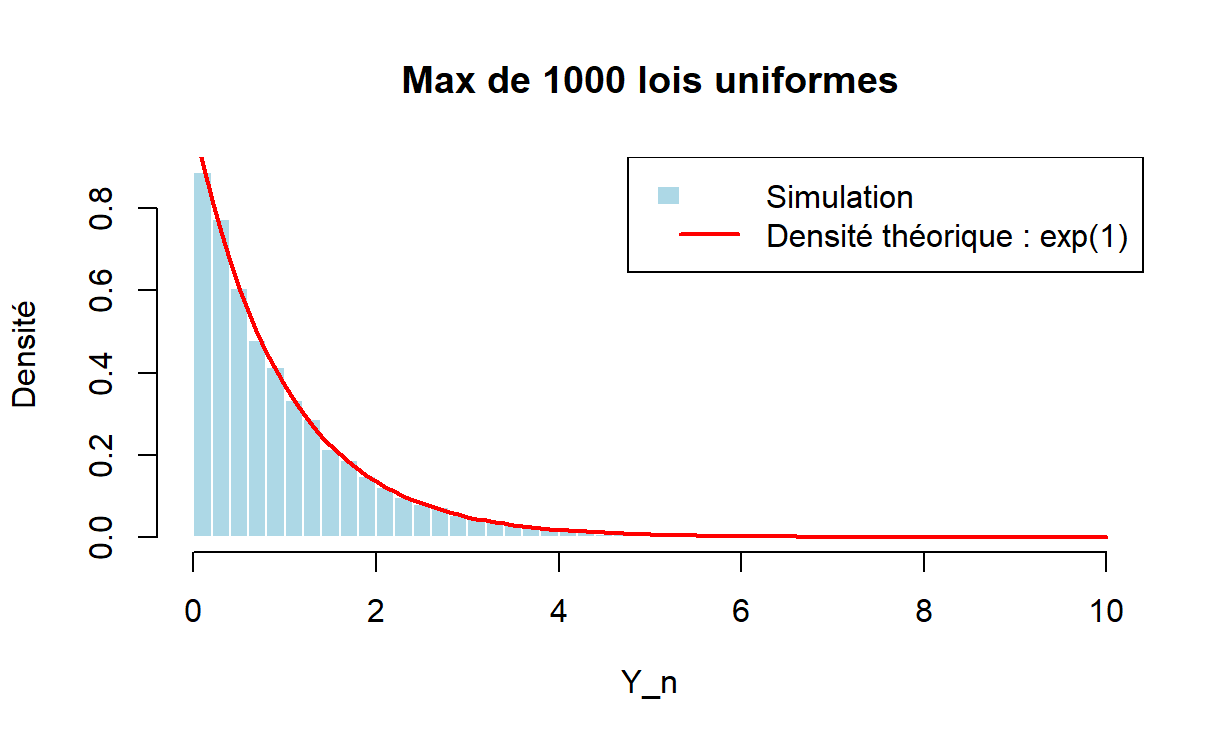
\includegraphics[scale=0.8]{./images/Max_Uniforme.png} 
\end{center}

\noindent Remarquons que l'on obtient une loi de Gumbell, ce qui est assez logique au vu du fait que ce soit une loi à queue très légère (elle n'en a tout simplement pas car son support est borné).

\subsubsection{Loi exponentielle}
\noindent Pour une loi exponentielle de paramètre 1, la loi limite est une loi de Gumbel. Théoriquement, on trouve $a_n = 1 $ et $b_n = \log(n) $.

\begin{center}
	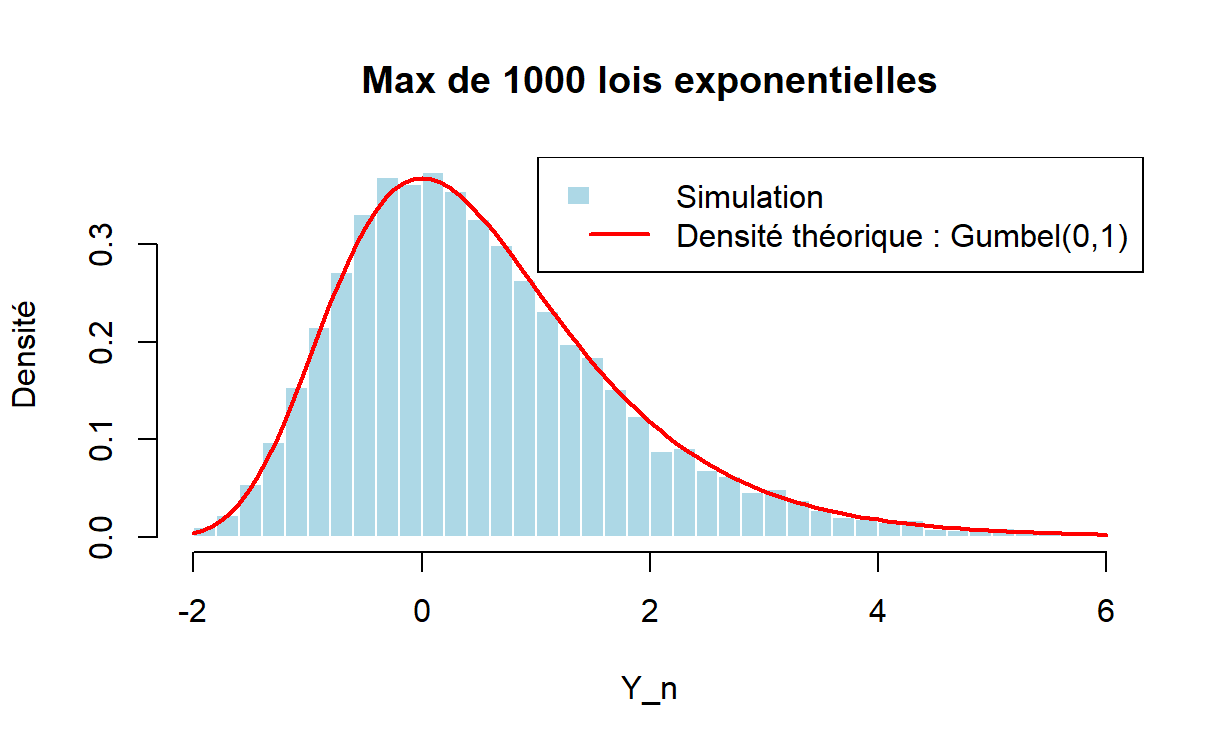
\includegraphics[scale=0.8]{./images/Max_Expo.png} 
\end{center}

\noindent Cette fois-ci, on avait une loi à queue fine, et on obtient loi de Gumbel, ce qui était attendu.

\subsubsection{Loi normale}

\noindent Pour maintenant une loi normale centrée-réduite, on peut montrer que la loi limite est encore une fois une loi de Gumbel. On trouve les paramètres généralisés $a_n = \frac{1}{\sqrt{(2*\log(n)}} $ et $b_n = \frac{1}{a_n} - \frac{\log(\log(n)) + \log(4 * pi)}{2 * \sqrt{2 * \log(n)}} $.

\begin{center}
	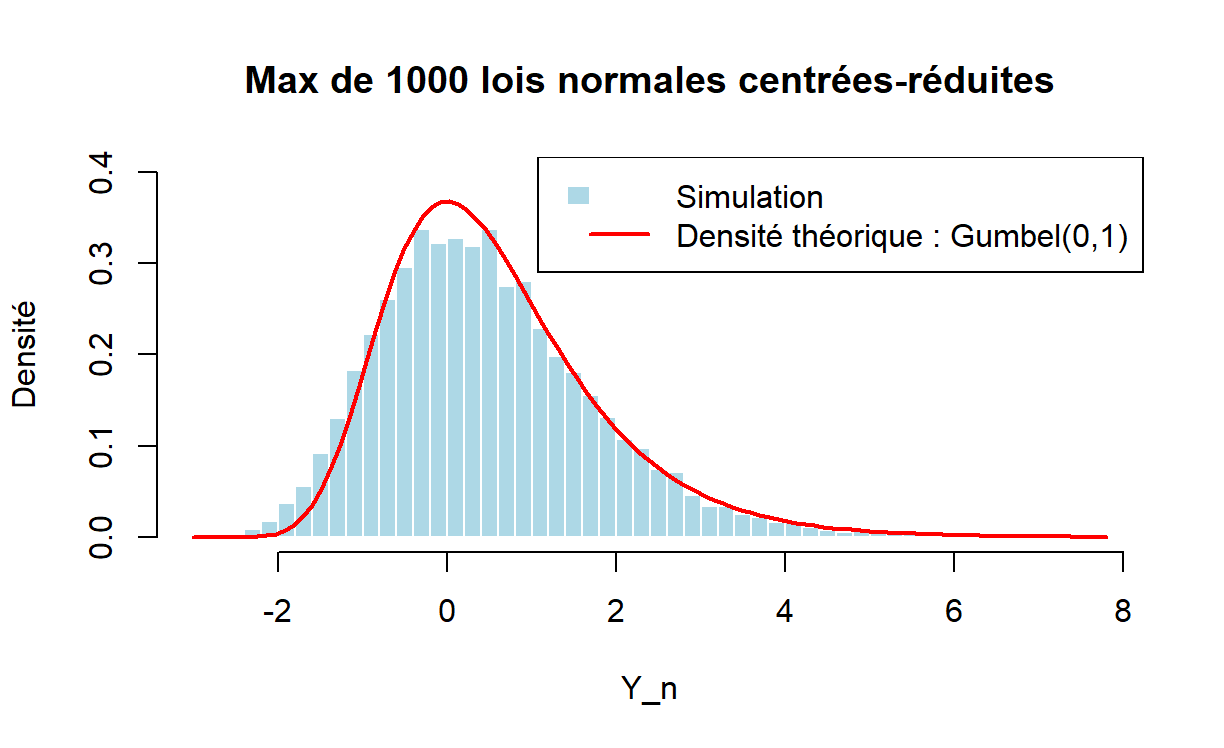
\includegraphics[scale=0.8]{./images/Max_Normale.png} 
\end{center}

\noindent Notons ainsi que l'on a la même loi limite que pour la loi exponentielle de paramètre 1, les graphes sont quasiment identiques.

\subsubsection{Loi de Cauchy}

\noindent Enfin, pour une loi de Cauchy (de paramètres 0 et 1 ici), la loi limite est une loi de Fréchet. On a les coefficients suivants : $a_n = pi $ et $b_n = n $.

\begin{center}
	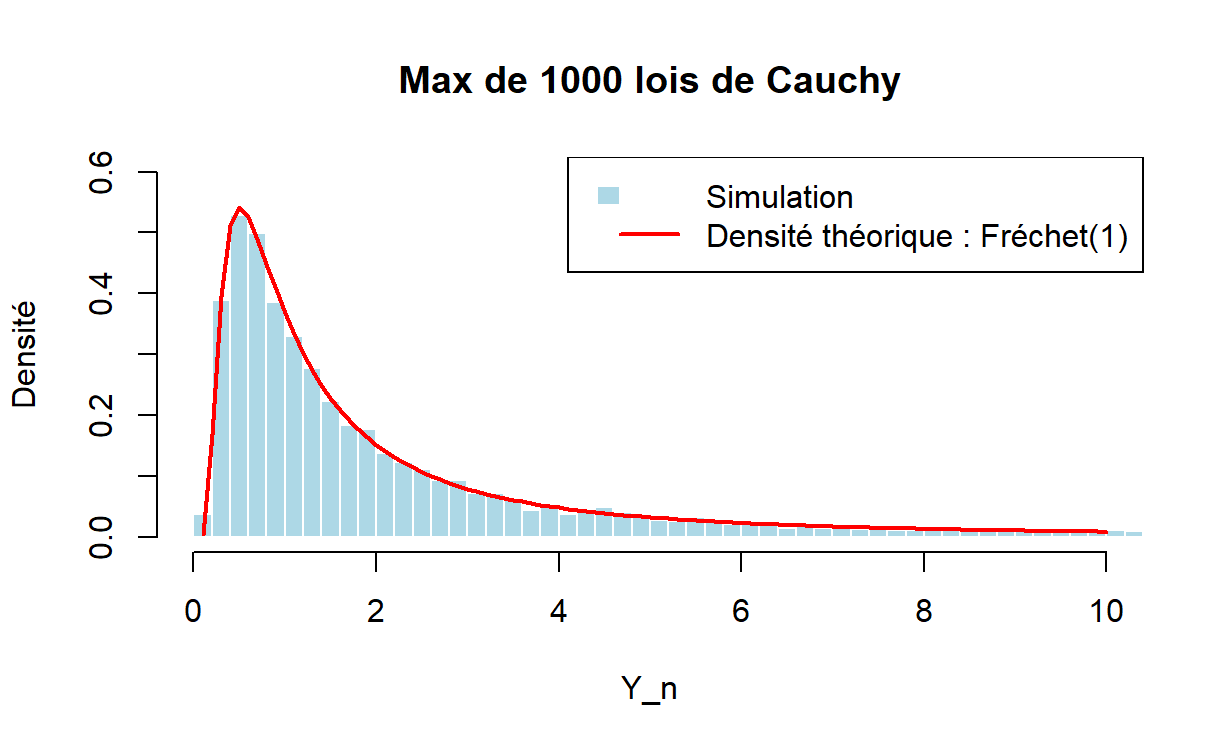
\includegraphics[scale=0.8]{./images/Max_Cauchy.png} 
\end{center}

\noindent Enfin ici, on avait une loi à queue lourde, et on obtient bien la loi de Fréchet attendue.

\newpage

\section{Méthodes d'estimation de l'indice de valeurs extrêmes}
Dans cette section, nous nous intéressons aux différentes méthodes d'estimation du paramètre \(\gamma\), intervenant dans la distribution des valeurs extrêmes généralisée. \\
D'une part, des approches non paramétriques sont dédiées à l'estimation de l'indice de queue, notamment les estimateurs de Hill et de Pickands. D'autre part, des méthodes paramétriques ont été développées, parmi lesquelles la méthode du maximum de vraisemblance, la méthode des moments et les approches bayésiennes. \\

\textbf{Définition :} On appelle \textit{statistique d'ordre} la permutation aléatoire de l'échantillon \(X_1, \dots, X_n\), qui ordonne les valeurs de l’échantillon par ordre croissant :

\[
X_{(1)} \leq X_{(2)} \leq \dots \leq X_{(n)}
\]

\textbf{Définition :} On dit qu'une suite \((k_n)_{n \geq 0}\) d'entiers est intermédiaire si :

\[
\lim_{n \to \infty} k_n = \infty \quad et \lim_{n \to \infty} \frac{k_n}{n} = 0
\]

\textbf{Définition :}
On dit qu'un estimateur \(\hat{\gamma_{n}}\) est convergent s'il converge en probabilité vers \(\gamma\), soit :
\[
\lim_{n \to \infty} P(\lvert \hat{\gamma_{n}} - \gamma \rvert > \epsilon) = 0 \quad \forall \epsilon > 0
\]

\subsection{Estimateur de Pickands}

L’estimateur de Pickands est construit à partir de trois statistiques d’ordre dans un échantillon. Il constitue l’un des premiers estimateurs non paramétriques proposés pour estimer l’indice des valeurs extrêmes \(\gamma\). Son principal avantage réside dans le fait qu’il est valide quel que soit le domaine d’attraction de la loi sous-jacente : Fréchet (\(\xi > 0\)), Gumbel (\(\xi = 0\)) ou Weibull (\(\xi < 0\)). Il n'est donc pas restreint à une famille particulière de distributions et reste applicable dans un cadre très général.

Néanmoins, cet estimateur est connu pour être assez sensible à la taille de l’échantillon, et en particulier au choix du paramètre intermédiaire \(k\), ce qui peut entraîner une certaine instabilité dans les estimations. Cela limite parfois sa robustesse, en particulier pour des tailles d’échantillon modestes.

En 1975, Pickands a démontré la consistance faible de son estimateur, c’est-à-dire la convergence en probabilité vers le vrai paramètre lorsque la taille de l’échantillon tend vers l’infini. Plus tard en 1989, Dekkers et de Haan ont établi la convergence forte ainsi que la normalité asymptotique de cet estimateur sous des conditions plus générales.

\medskip
\textbf{Définition.} Soit \(X_1, \dots, X_n\) une suite de variables aléatoires i.i.d. de loi \(F\), appartenant à l’un des domaines d’attraction des lois de valeurs extrêmes. On note \(X_{1,n} \leq \dots \leq X_{n,n}\) les statistiques d’ordre croissantes. Soit \((k_n)_{n \geq 1}\) une suite intermédiaire telle que \(k_n \to \infty\) et \(k_n / n \to 0\), l’estimateur de Pickands est défini par :

\[
\hat{\gamma}_{k,n} = \frac{1}{\ln(2)} \ln\left( \frac{X_{n-k+1,n} - X_{n-2k+1,n}}{X_{n-2k+1,n} - X_{n-4k+1,n}} \right)
\]

\medskip
L’estimateur de Pickands repose sur l’idée que, dans les queues d’une distribution extrême, les plus grandes observations suivent un comportement régulier. En considérant des statistiques d’ordre décroissantes, on peut approximer la structure de la queue à l’aide de différences successives entre grandes valeurs. L’utilisation d’une transformation logarithmique permet alors d’isoler l’indice de queue \(\gamma\), sous des conditions d’attraction à une loi limite.

\medskip
\textbf{Propriété de consistance.} Si \((k_n)\) est une suite intermédiaire, alors :
\[
\hat{\gamma}_{k,n} \xrightarrow{\mathbb{P}} \gamma
\quad \text{lorsque } n \to \infty.
\]

De plus, sous hypothèses régulières, l’estimateur est asymptotiquement normal :
\[
\sqrt{k} \left( \hat{\gamma}_{k,n} - \gamma \right) \xrightarrow{\mathcal{L}} \mathcal{N}(0, \sigma^2(\gamma))
\]
où la variance asymptotique est donnée par :
\[
\sigma(\gamma) = \frac{\gamma \sqrt{2^{2\gamma + 1} + 1}}{2(2^{\gamma} - 1)\ln(2)}.
\]

\medskip
Cette formule théorique permet de construire des intervalles de confiance pour l’estimation de \(\gamma\), bien qu’en pratique la variance soit souvent estimée par simulation.

\medskip
Enfin, une version généralisée de cet estimateur existe, introduisant deux paramètres \(u, v > 1\), permettant une plus grande flexibilité :
\[
\hat{\gamma}_{(k,u,v)} = \frac{1}{\ln(v)} \ln\left( \frac{X_{n-k+1,n} - X_{n-[uk]+1,n}}{X_{n-[vk]+1,n} - X_{n-[uvk]+1,n}} \right)
\]
Cette généralisation permet d'ajuster la stabilité de l'estimation. On retrouve l'estimateur de Pickands classique en prenant \(u = v = 2\).

\subsection{Représentation graphique de l’estimateur de Pickands}

Afin d'illustrer le comportement de l’estimateur de Pickands dans différents contextes, nous l'appliquons à des échantillons simulés de taille \(n = 40\,000\), issus de quatre lois représentatives : la loi de Pareto, la loi exponentielle, la loi uniforme sur \([0,1]\), et la loi de Cauchy. Ces lois permettent de couvrir les trois domaines d’attraction des lois de valeurs extrêmes, avec des indices théoriques respectifs de queue \(\gamma\) valant \(0.5\), \(0\), \(-1\), et \(1\).

Les figures ci-dessous présentent l’évolution de l’estimateur \(\hat{\gamma}_{k,n}\) en fonction de \(k\), c’est-à-dire du nombre d’observations extrêmes utilisées dans le calcul. Une ligne rouge horizontale indique la valeur théorique de \(\gamma\) pour chaque distribution, afin de visualiser la qualité de convergence.

\subsubsection{Loi de Pareto (\(\alpha = 2\))}

\begin{figure}[H]
    \centering
    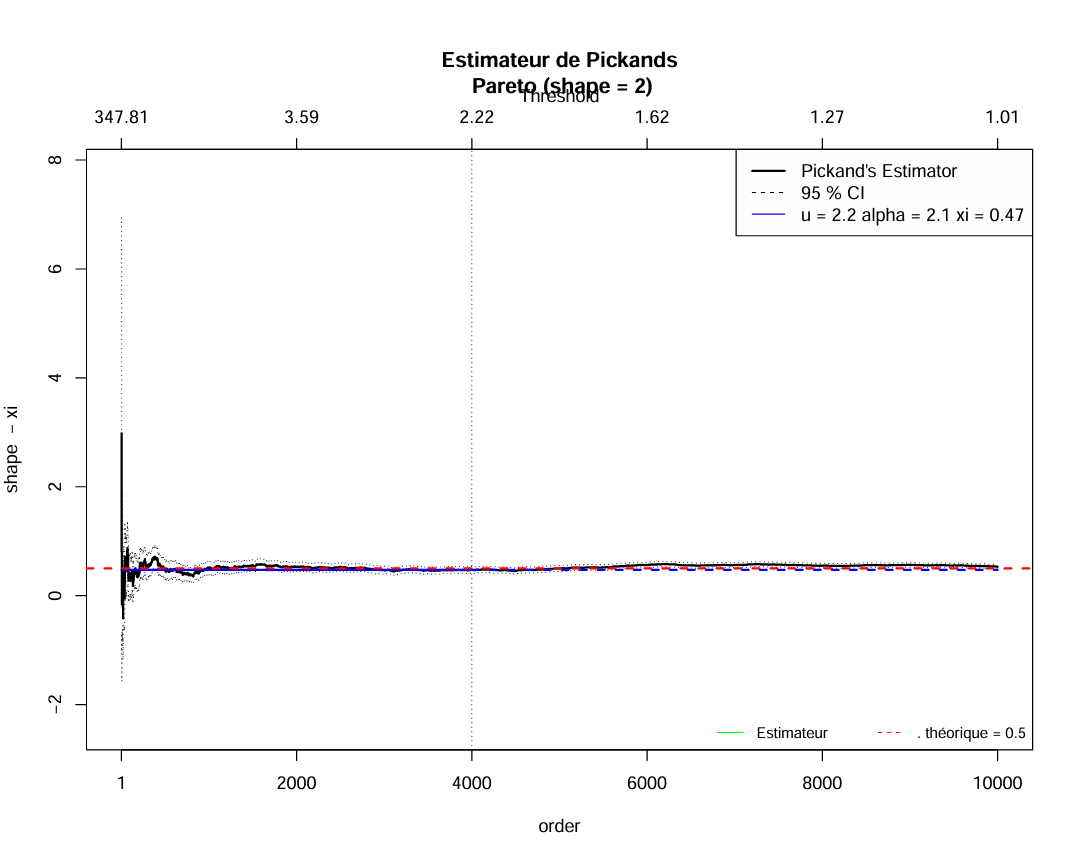
\includegraphics[width=0.8\textwidth]{./images/pareto.png}
    \caption{Estimateur de Pickands pour la distribution de Pareto (shape = 2).}
    \label{fig:pickands_pareto}
\end{figure}

La figure \ref{fig:pickands_pareto} illustre l’estimateur de Pickands appliqué à un échantillon simulé selon une loi de Pareto de paramètre \(\alpha = 2\), ce qui correspond à un indice de queue \(\gamma = 1/\alpha = 0.5\). L’estimateur converge clairement vers cette valeur lorsque \(k\) augmente, ce qui confirme la bonne performance de l’estimateur dans le cas d’une distribution à queue lourde.

\subsubsection{Loi exponentielle}

\begin{figure}[H]
    \centering
    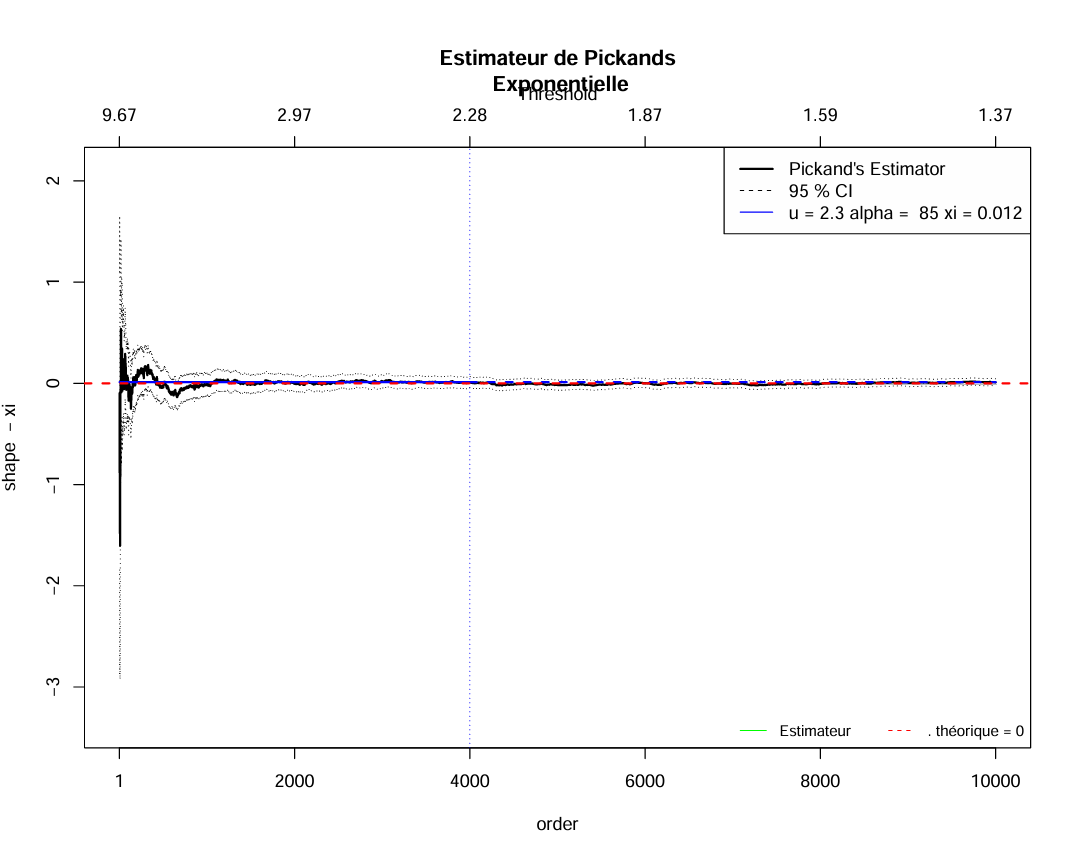
\includegraphics[width=0.8\textwidth]{./images/exponentielle.png}
    \caption{Estimateur de Pickands pour la distribution exponentielle.}
    \label{fig:pickands_exponentielle}
\end{figure}

Dans la figure \ref{fig:pickands_exponentielle}, on observe que l’estimateur de Pickands reste proche de zéro, en accord avec l’indice théorique \(\gamma = 0\) de la loi exponentielle. Ce résultat est cohérent avec le fait que cette loi appartient au domaine d’attraction de Gumbel.
\subsubsection{Loi uniforme \([0,1]\)}

\begin{figure}[H]
    \centering
    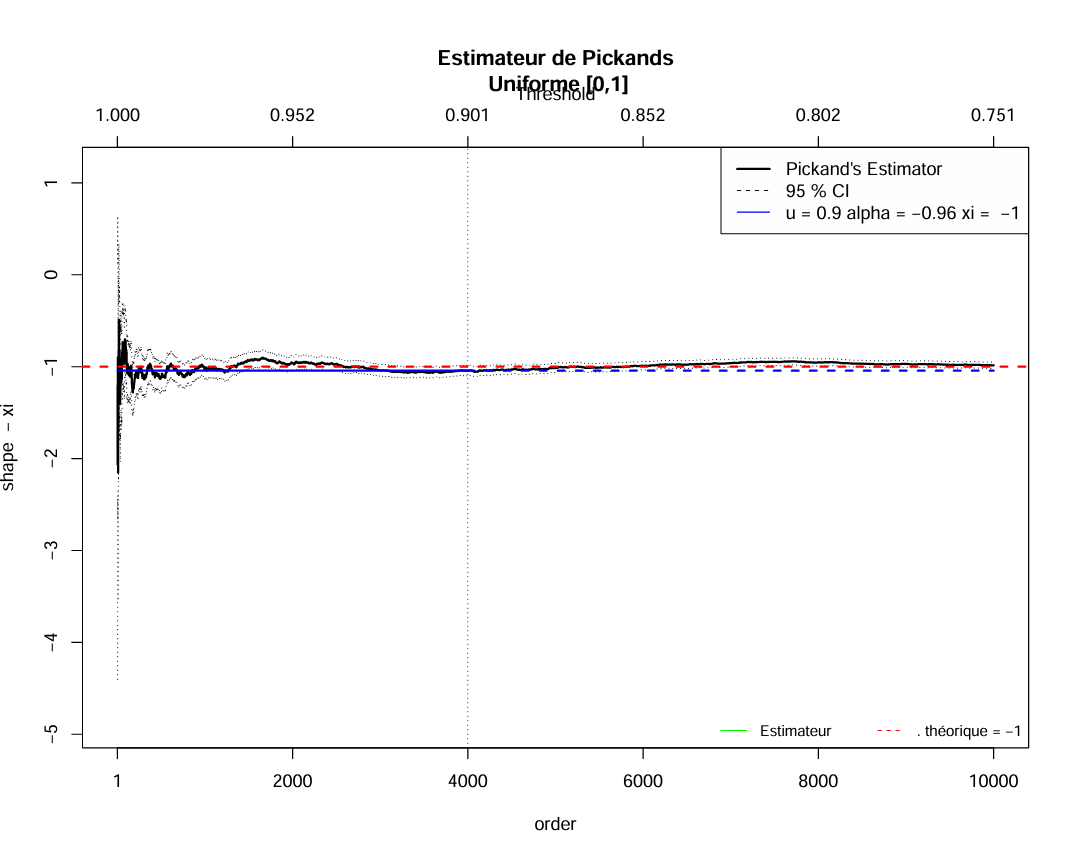
\includegraphics[width=0.8\textwidth]{./images/uniforme.png}
    \caption{Estimateur de Pickands pour la distribution uniforme sur \([0,1]\).}
    \label{fig:pickands_uniforme}
\end{figure}

Comme le montre la figure \ref{fig:pickands_uniforme}, l’estimateur décroît vers \(\gamma = -1\), valeur attendue pour la loi uniforme qui possède une queue bornée. La plus grande instabilité observée est due au fait que cette loi n’a pas de queue lourde, ce qui affecte la stabilité de l’estimation.

\subsubsection{Loi de Cauchy}

\begin{figure}[H]
    \centering
    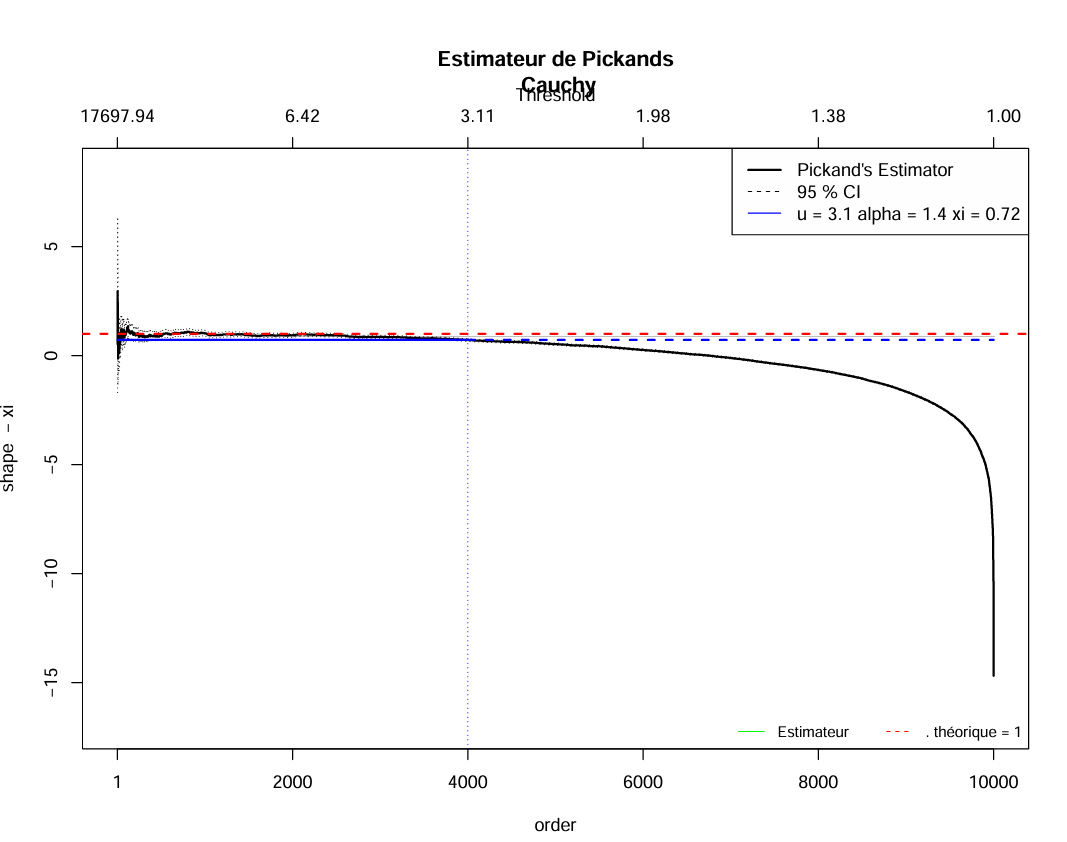
\includegraphics[width=0.8\textwidth]{./images/cauchy.png}
    \caption{Estimateur de Pickands pour la distribution de Cauchy.}
    \label{fig:pickands_cauchy}
\end{figure}

La figure \ref{fig:pickands_cauchy} présente l’estimateur de Pickands appliqué à un échantillon de loi de Cauchy. Cette loi est caractérisée par une queue extrêmement lourde et appartient au domaine d’attraction de Fréchet, avec un indice de queue théorique \(\gamma = 1\).

Le comportement de l’estimateur est ici particulièrement intéressant. Pour les faibles valeurs de \(k\), l’estimateur est très instable, ce qui est attendu compte tenu de la nature explosive des grandes valeurs dans une loi de Cauchy. À partir d’un certain seuil (environ \(k = 500\)), une phase de stabilisation est visible, avec une estimation qui reste relativement proche de la valeur attendue.

Cependant, on note qu’au-delà de \(k \approx 4000\), l’estimateur décroît significativement. Cela s’explique par le fait que l’inclusion d’observations moins extrêmes perturbe la qualité de l’estimation.
Ainsi, le cas de la Cauchy montre bien les limites pratiques de l’estimateur, malgré sa validité théorique.

\subsubsection{Synthèse}
Ces représentations graphiques montrent que l’estimateur de Pickands parvient globalement à capturer l’indice de queue \(\gamma\) pour différentes familles de distributions. Il converge correctement pour les cas classiques (Pareto, exponentielle), mais présente une instabilité accrue pour les queues bornées ou très lourdes. Ces résultats illustrent à la fois les points forts et les limites de l’estimateur, notamment sa sensibilité au choix de \(k\).

\subsection{Construction de l'estimateur de Pickands}
\textbf{Proposition :} (Caractérisations de \( D(H_{\gamma}) \))

Pour \( \gamma \in \mathbb{R} \), les affirmations suivantes sont équivalentes. \newline
\( (a) \quad F \in D(H_{\gamma}) \) \newline
\( (b) \) Pour une certaine fonction positive \( c(t) = a\left( \frac{1}{t} \right) \) :

\[
\lim_{t \to 0} \frac{U(tx) - U(t)}{c(t)} = 
\begin{cases} 
\frac{x^\gamma - 1}{\gamma} & \text{si } \gamma \neq 0, \\
\log(x) & \text{si } \gamma = 0, 
\end{cases}
\quad \text{pour } x > 0.
\]
La dernière affirmation est équivalente à :
\[
\lim_{s \to 0} \frac{U(sx) - U(s)}{U(sy) - U(s)} = 
\begin{cases} 
\frac{x^\gamma - 1}{y^\gamma - 1} & \text{si } \gamma \neq 0, \\
\frac{\log(x)}{\log(y)} & \text{si } \gamma = 0.
\end{cases}
\]
pour \(x,y > 0\) et \(y \neq 1\). \newline

\textbf{Lemme A:}
Soit \(X_1, \dots, X_n\) des variables aléatoires indépendantes et de fonction de répartition \(F\).
Soit \(U_1, \dots, U_n\) des variables aléatoires indépendantes de loi uniforme \(\left[0,1\right]\). Alors \(F^{-1}(U_{1,n}), \dots, F^{-1}(U_{n,n})\) a même loi que \((X_{1,n}, \dots, X_{n,n})\)\newline
\textbf{Preuve de la construction de l'estimateur de Pickands :}

On déduit de la proposition précédente que pour $\gamma \in \mathbb{R}$ et $\alpha$ on a avec le choix $t = 2s$, $x = 2$ et $y = \frac{1}{2}$,
\[
\lim_{t \to \infty} \frac{U(t) - U(t/2)}{U(t/2) - U(t/4)} = 2^{\gamma}.
\]

En fait, en utilisant la croissance de $U$ qui se déduit de la croissance de $F$, on obtient
\[
\lim_{t \to \infty} \frac{U(t) - U(t_{c_1}(t))}{U(t_{c_1}(t)) - U(t_{c_2}(t))} = 2^{\gamma}
\]
dès que $\lim_{t \to \infty} c_1(t) = \frac{1}{2}$ et $\lim_{t \to \infty} c_2(t) = \frac{1}{4}$. Il reste donc à trouver des estimateurs pour $U(t)$.

Soit $k(n), n \geq 1$ une suite d’entiers telle que $1 \leq k(n) \leq \frac{n}{4}$ et $\lim_{n \to \infty} \frac{k(n)}{n} = 0$ et $\lim_{n \to \infty} k(n) = \infty$.

Soit $(V_{1,n},\dots,V_{n,n})$ la statistique d’ordre d’un échantillon de variables aléatoires indépendantes de loi de Pareto. On note $F_V(x) = 1 - x^{-1}, x \geq 1$.

On déduit avec certains résultats de bases liés à $(V_{1,n},\dots,V_{n,n})$ que les suites
\[
\frac{k}{n} V_{n-k+1,n}, \quad \frac{2k}{n} V_{n-2k+1,n}, \quad \frac{4k}{n} V_{n-4k+1,n}
\]
pour \(n \geq 1\) convergent en probabilité vers 1.

On en déduit en particulier, les convergences en probabilité suivantes :
\[
V_{n-k+1,n}  \to \infty, \quad \frac{V_{n-2k+1,n}}{V_{n-k+1,n}} \to \frac{1}{2}, \quad \frac{V_{n-4k+1,n}}{V_{n-k+1,n}} \to \frac{1}{4}.
\]

Donc la convergence suivante a lieu en probabilité :
\[
\frac{U(V_{n-k+1,n}) - U(V_{n-2k+1,n})}{U(V_{n-2k+1,n}) - U(V_{n-4k+1,n})} \to 2^{\gamma}.
\]

Remarquons que si $x \geq 1$, alors $U(x) = F^{-1}(F_V(x))$. On a donc
\[
(U(V_{1,n}), \dots, U(V_{n,n})) = (F^{-1}(F_V(V_{1,n})), \dots, F^{-1}(F_V(V_{n,n}))).
\]

Or \(F_V\) est la fonction de répartition de la loi de Pareto. \newline
On déduit de la croissance de $F_V$ que $(F^{-1}(F_V(V_{1,n})),\dots, F^{-1}(F_V(V_{n,n})))$ a la même loi qu’une suite de $n$ variables aléatoires uniformes sur $[0,1]$ indépendantes. 

On déduit du lemme A que le vecteur aléatoire $(F^{-1}(F_V(V_{1,n})),\dots, F^{-1}(F_V(V_{n,n})))$ a la même loi que $(X_1,\dots,X_n)$. 

Donc la variable aléatoire \(\frac{U(V_{n-k+1,n}) - U(V_{n-2k+1,n})}{U(V_{n-k+1,n}) - U(V_{n-4k+1,n})}\) a la même loi que :

\[
\frac{X_{n-k+1,n} - X_{n-2k+1,n}}{X_{n-k+1,n} - X_{n-4k+1,n}}
\]

Ainsi cette quantité converge en loi vers $2^{\gamma}$ quand $n$ tend vers l’infini.

\subsection{Estimateur de Hill}
Cet estimateur a été introduit par Hill en 1975 dans le but d’estimer, de manière non paramétrique, le paramètre de queue des lois appartenant au domaine d’attraction de Fréchet. Il offre une estimation de l’indice de queue généralement plus efficace que celle fournie par l’estimateur de Pickands. La construction de cet estimateur repose sur l’utilisation des $k_n$ plus grandes statistiques d’ordre de l’échantillon.


\subsection{quantile de retour}

En pratique, on cherche une valeur qui donnerait une certaine confiance quand à l'apparition
de données la depassant. Dans le cas d'une distribution à queue bornée il suffit de prendre la bornes supérieure de la distribution.
\\
Or, dans le cas d'une distribution à queue lourde et exponentiel ce n'est pas possible. On introduit alors la notion de \textbf{quantile de retour} qui est une valeur que l'on dépasse en moyenne une fois tous les T ans.
\\
On pose $z_T$ cette quantité, et elle est solution de l'équation suivante :
\[
P\bigl(M \le z_T\bigr)
\;=\;
G_{\mu,\sigma,\gamma}(z_T)
\;=\;
1 - \frac{1}{T},
\]
où \(G_{\mu,\sigma,\gamma}\) est la fonction de répartition de la GEV. En résolvant cette équation que l'on admet, on obtient
\[
z_T =
\begin{cases}
\displaystyle
\mu \;+\;\frac{\sigma}{\gamma}\Bigl[(-\ln(1 - 1/T))^{-\gamma} - 1\Bigr],
&\gamma \neq 0,\\[1em]
\displaystyle
\mu \;-\;\sigma\,\ln\bigl(-\ln(1 - 1/T)\bigr),
&\gamma = 0.
\end{cases}
\]
\section{La construction de l’estimateur de Hill}

Soient $\alpha_n$ et $\beta_n$ deux suites de nombres positifs, la construction de l’estimateur de Hill basée sur la relation suivante :

\begin{equation}
    q_{\beta_n} \simeq q_{\alpha_n} \left( \frac{\alpha_n}{\beta_n} \right)^{\gamma}.
    \tag{1.6}
\end{equation}

Passons au logarithme dans l’équation (1.6), ce qui donne :

\[
\log(q_{\beta_n}) - \log(q_{\alpha_n}) \simeq \gamma \log\left( \frac{\alpha_n}{\beta_n} \right).
\]

On choisit $\alpha_n = k_n/n$ et on considère plusieurs valeurs pour $\beta_n$, $\beta_n = i/n$ avec $i = 1, \ldots, k_n - 1$ tout en ayant $\beta_n < \alpha_n$. On obtient alors :

\[
\log(q_{i/n}) - \log(q_{k_n/n}) \simeq \gamma \log(k_n/i).
\]

Ainsi, en estimant les quantiles par leurs équivalents empiriques, on obtient :

\[
\log(X_{n - i + 1, n}) - \log(X_{n - k_n + 1, n}) \simeq \gamma \log(k_n / i).
\]

En sommant de part et d’autre sur $i = 1, \ldots, k_n - 1$, on obtient :

\[
\gamma = \frac{\displaystyle \sum_{i=1}^{k_n - 1} \log(X_{n - i + 1, n}) - \log(X_{n - k_n + 1, n})}{\displaystyle \sum_{i=1}^{k_n - 1} \log(k_n / i)}.
\]

Le dénominateur se réécrit $\log(k_n^{k_n - 1}/(k_n - 1)!)$. En utilisant la formule de Stirling, il est équivalent à $k_n$ au voisinage de l’infini. On obtient alors l’estimateur de Hill.

Soit $(k_n)_{n \geq 1}$ une suite d'entiers avec $1 \leq k_n \leq n$, l’estimateur de Hill est défini par :

\[
\hat{\gamma}^{H}_{k_n} = \frac{1}{k_n - 1} \sum_{i=1}^{k_n - 1} \log(X_{n - i + 1, n}) - \log(X_{n - k_n + 1, n}).
\]

L’estimateur de Hill satisfait la propriété de consistance faible. Plus précisément, si $(k_n)_{n \geq 1}$ est une suite intermédiaire, alors l’estimateur $\hat{\gamma}^{H}_{k_n}$ converge en probabilité vers le paramètre de queue $\gamma$, c’est-à-dire :
\[
\hat{\gamma}^{H}_{k_n} \xrightarrow{\mathbb{P}} \gamma.
\]


\subsection{Le choix du nombre de statistiques d’ordre}

Dans la pratique, déterminer une valeur appropriée pour le paramètre $k_n$, c’est-à-dire le nombre de plus grandes observations à retenir, constitue une étape délicate. Il faut en effet trouver un compromis entre la variance et le biais : utiliser suffisamment de données pour obtenir une estimation fiable, tout en s’assurant que ces données proviennent bien de la queue de la distribution. Diverses approches ont été développées dans la littérature pour guider ce choix.

\subsection{Comportement empirique de l’estimateur de Hill}

Nous présentons ci-dessous des représentations graphiques de l’estimateur de Hill appliqué à des échantillons de taille $n = 40000$ générés à partir de quatre lois différentes : Pareto, exponentielle, uniforme et Cauchy. Pour chacune d’elles, nous comparons les valeurs estimées de l’indice de queue $\gamma$ à leur valeur théorique.

\paragraph{Loi de Pareto :}
\begin{figure}[H]
    \centering
    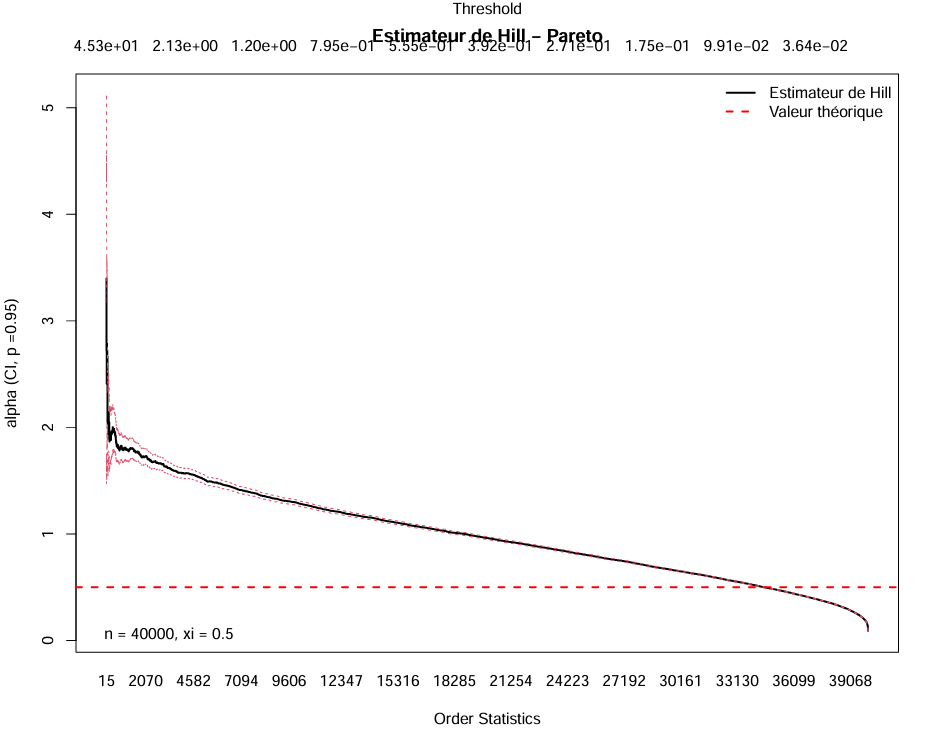
\includegraphics[width=0.6\textwidth]{./images/hill_pareto.png}
    \caption{Estimateur de Hill — Loi de Pareto ($\gamma = 0{,}5$)}
\end{figure}

Dans ce cas, la loi suit un comportement de queue lourde avec un indice théorique $\gamma = 0.5$, ce qui correspond parfaitement aux hypothèses de l’estimateur de Hill. Comme le montre la Figure, l’estimation converge de manière satisfaisante vers la valeur théorique pour un intervalle raisonnable de seuils $k$. On observe une certaine instabilité pour les petites valeurs de $k$, mais une fois la courbe stabilisée, elle oscille autour de la vraie valeur. Ce comportement valide l'efficacité de l’estimateur dans ce cadre.
\paragraph{Loi exponentielle :}
\begin{figure}[H]
    \centering
    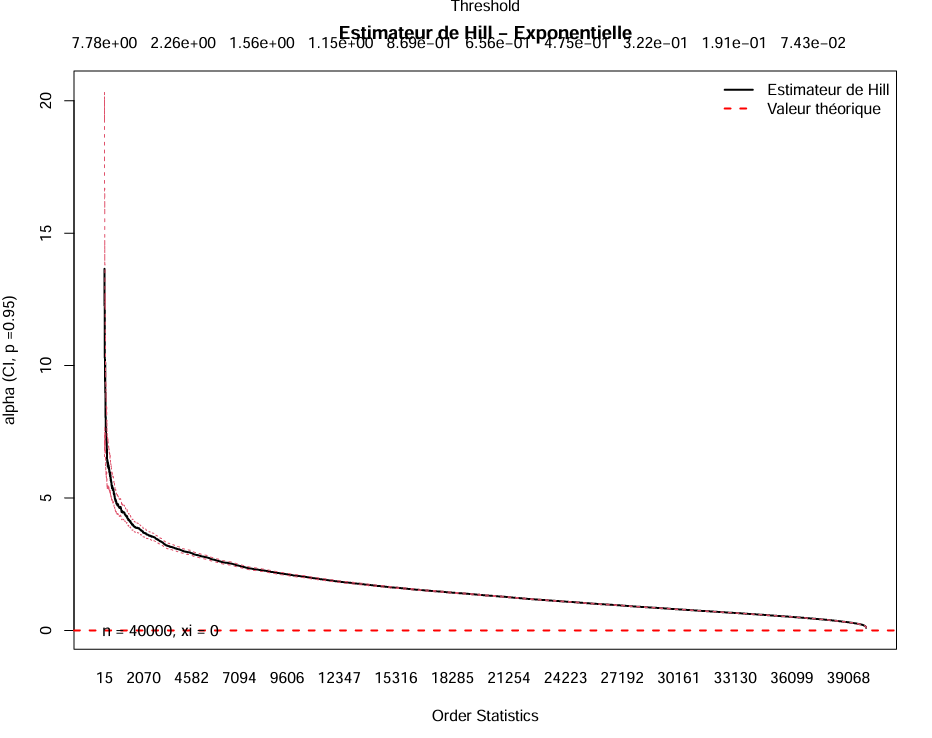
\includegraphics[width=0.6\textwidth]{./images/hill_expo.png}
    \caption{Estimateur de Hill — Loi exponentielle ($\gamma = 0$)}
\end{figure}

La loi exponentielle appartient au domaine de Gumbel, avec un indice de queue $\gamma = 0$. L’estimateur de Hill n’est pas adapté à ce domaine. Le graphique le confirme clairement : la courbe estimée commence avec des valeurs très élevées, puis décroît lentement sans jamais converger vers la valeur théorique nulle. L’absence de convergence met en évidence l’inadéquation de l’estimateur dans ce contexte.
\paragraph{Loi uniforme :}
\begin{figure}[H]
    \centering
    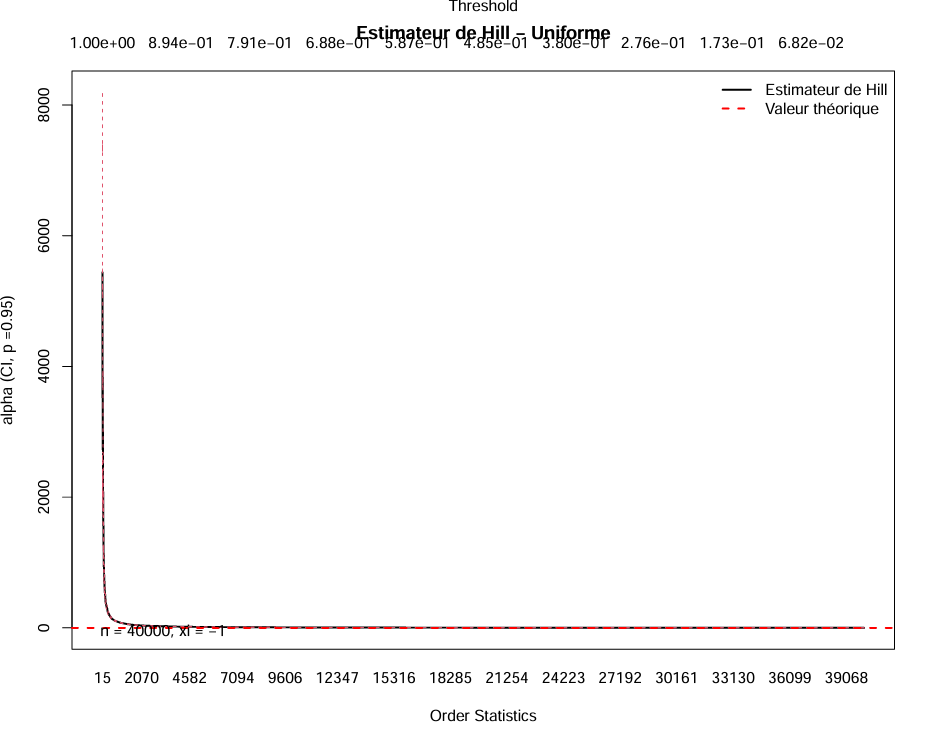
\includegraphics[width=0.6\textwidth]{./images/hill_uniforme.png}
    \caption{Estimateur de Hill — Loi uniforme ($\gamma = -1$)}
\end{figure}

Cette loi présente une queue bornée, avec un indice $\gamma = -1$, ce qui sort du domaine d’application de Hill. L’estimateur suppose en effet que $\gamma > 0$. Le graphique montre une estimation extrêmement instable, avec des valeurs incohérentes, souvent très grandes ou très faibles, indiquant que le modèle n’est pas du tout approprié à ce type de données. 
\paragraph{Loi de Cauchy :}
\begin{figure}[H]
    \centering
    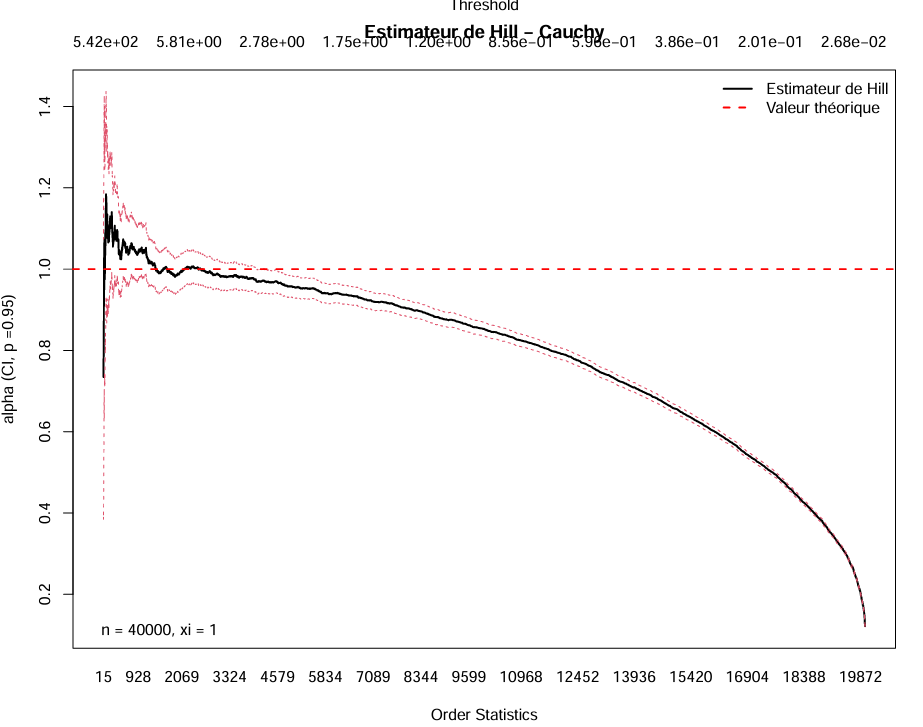
\includegraphics[width=0.6\textwidth]{./images/hill_cauchy.png}
    \caption{Estimateur de Hill — Loi de Cauchy ($\gamma = 1$)}
\end{figure}

La distribution de Cauchy, avec un indice $\gamma = 1$, est dans le domaine de Fréchet, donc en principe bien adaptée à l’estimateur de Hill. Le graphique montre une bonne estimation dans les faibles valeurs de $k$, la courbe noire se stabilisant autour de la valeur théorique. Cependant, dès que $k$ devient trop grand, l’estimation chute fortement, trahissant un biais introduit par l'inclusion d’observations moins extrêmes. Ce phénomène illustre la sensibilité de l’estimateur au choix du seuil $k$.
\medskip

En résumé, ces observations soulignent la pertinence de l’estimateur de Hill pour les lois à queue lourde (Pareto, Cauchy), et son inadéquation manifeste pour les lois à queue légère ou bornée (exponentielle, uniforme). Le choix judicieux du paramètre $k$ demeure également crucial pour obtenir une estimation fiable.

\section{Méthode des maxima par blocs}

\noindent L'approche des maxima par blocs (en anglais Blocks Maxima) consiste à diviser les n observations en N blocs de taille k. Concrètement, la suite $X_1, ..., X_n$ est divisée en N blocs, le premier bloc est $X_1, ..., X_k$, le second $X_{k+1}, ..., X_{2k}$, etc. On obtient ainsi une suite de maxima $M_1, ..., M_n$ définis sur chacun des blocs.\\
\noindent En général, on considère une période temporelle, comme une journée ou bien une année pour refléter le sens des observations.  \\
\noindent On peut alors déterminer la loi limite des maxima, en vertu du théorème de Fisher-Tippett-Gnedenko c'est une distribution GEV classique de la forme :
\[
G_{\mu,\sigma,\gamma}(x)
\;=\;
\exp\!\Bigl\{-\bigl[1 + \gamma\,u\bigr]^{-1/\gamma}\Bigr\}.
\]

\noindent De la même manière que ce que l'on avait sans les blocs, il faut alors déterminer les valeurs des paramètres en les approximant par des méthodes comme le maximum de vraisemblance. Des auteurs comme Ferreira et de Haan (2006 et 2015) ont alors démontré l'existence d'estimateurs pertinents pour cette méthode, nommés PWM (pour "probability weighted moment"). Pour les définir, on part de la statistique suivante, soient $X_{1,k}, ..., X_{k,k}$ les observations ordonnées du bloc $X_1, ..., X_k$, on définit :
\[
\beta_r = \frac{1}{k} \sum_{i=1}^{k} \frac{(i-1)...(i-r)}{(k-1)...(k-r)} X_{i,k} ~ \text{ pour $r = 1,2,3,...,k>r $}
\] \\
\noindent A partir de $\beta_r$, on peut ensuite définir les trois estimateurs PVM suivants pour $\gamma, a_n$ et $b_n$ qui possèdent de bonnes propriétés asymptotiques sous certaines conditions ($\Gamma$ est la fonction gamma d'Euler). \\

\noindent Pour $\gamma$ : $\hat{\gamma}_{k,m}$ est solution de $\frac{3\hat{\gamma}_{k,m} - 1}{2\hat{\gamma}_{k,m} - 1} = \frac{3\beta_2 - \beta_0}{2\beta_1 - \beta_0} $ \\
\noindent Pour $a_n$ : $\hat{a}_{k,m} = \frac{\hat{\gamma}_{k,m}}{2\hat{\gamma}_{k,m} - 1} \cdot \frac{2\beta_1 - \beta_0}{\Gamma(1 - \hat{\gamma}_{k,m})}$ \\
\noindent Pour $b_n$ : $\hat{b}_{k,m} = \beta_0 + \hat{a}_{k,m} \cdot \frac{1 - \Gamma(1 - \hat{\gamma}_{k,m})}{\hat{\gamma}_{k,m}}$ \\

\noindent Sous certaines conditions, on peut enfin démontrer que les quantiles élevés sont estimables par cette méthode. On a ainsi :
\[
\frac{\sqrt{k} \left( \hat{X}_{k,m} - X_n \right)}{a_n \, q_{\gamma}(c_n)}
\xrightarrow{d}
\Delta + (\gamma^-)^2 B - \gamma^- \Lambda - \lambda \frac{\gamma^-}{\gamma^- + \rho}
\]
où : \begin{itemize}
	\item $\hat{X}_{k,m}$ est l’estimateur du quantile extrême
	\item $X_n$ est le vrai quantile à estimer
	\item $a_n$ est le paramètre d'échelle
	\item $\Delta, \Lambda, \lambda$ sont des paramètres issus de la théorie asymptotique de Ferreira et de Haan (2015)
	\item $B$ est un pont brownien
	\item $q_{\gamma}(c_n)$ est une fonction définie par $q_{\gamma}(t) = \int_1^t s^{\gamma - 1} \log s \, ds$
	\item $\gamma^- = \min(0, \gamma)$
\end{itemize}
\vspace{0.5cm}
\noindent Cette approche possède tout de même un défaut car lorsque l'on prend le maximum sur un bloc, on fait potentiellement disparaître des valeurs élevées, on perd des données intéressantes.

\section{Méthode des excès}

La méthode des excès, également appelée approche par dépassement de seuil (en anglais \textit{Peaks Over Threshold}, ou POT), a été introduite par Pickands en 1975. Elle constitue une alternative à l’approche classique par blocs pour modéliser les phénomènes extrêmes.

Le principe est de ne conserver que les observations excédant un seuil élevé \( u \). Si ce seuil est bien choisi la distribution des excès définis par :
\[
Y_i = X_i - u \quad \text{pour} \quad X_i > u
\]
peut être approximée par une distribution de Pareto généralisée (GPD).

\medskip
Cette approche repose sur un résultat fondamental de Balkema et de Haan (1974), et de Pickands (1975), selon lequel, pour une grande classe de lois de probabilité \(F\), la loi des excès conditionnels au-delà d’un seuil élevé converge vers une loi de Pareto généralisée lorsque le seuil \(u\) tend vers la borne supérieure de \(F\).

\medskip
Formellement, on considère une suite de variables aléatoires i.i.d. \(X_1, \dots, X_n\) de fonction de répartition \(F\), et \(x_F\) le point terminal de \(F\). Pour tout seuil \(u < x_F\), on définit la fonction de répartition des excès par :

\[
F_u(x) := \mathbb{P}(X - u \leq x \mid X > u) = \frac{F(x + u) - F(u)}{1 - F(u)},
\quad \text{pour } 0 \leq x \leq x_F - u.
\]

Et sa version en fonction de survie :
\[
\overline{F}_u(x) := \mathbb{P}(X - u > x \mid X > u) = \frac{\overline{F}(x + u)}{\overline{F}(u)}.
\]

Lorsque le seuil \(u\) est suffisamment élevé, \(F_u\) peut être bien approchée par une distribution de Pareto généralisée \(G_{\gamma, \beta(u)}\), définie comme suit :

\subsection{Loi de Pareto généralisée (GPD)}

La fonction de répartition de la GPD est donnée par :

\[
G_{\gamma, \beta}(y) =
\begin{cases}
1 - \left(1 + \dfrac{\gamma y}{\beta}\right)^{-1/\gamma}, & \text{si } \gamma \neq 0, \\
1 - \exp\left(-\dfrac{y}{\beta}\right), & \text{si } \gamma = 0,
\end{cases}
\]
avec \( y \geq 0 \), sous la condition \(1 + \gamma y/\beta > 0\). Le paramètre \(\beta > 0\) représente l’échelle et \(\gamma\) le paramètre de forme (indice de queue).

\medskip
\textbf{Exemple (cas exponentiel)}.\\
Soit \(F(x) = 1 - e^{-x}\) la loi exponentielle standard. On a pour tout \(y > 0\) :

\[
\mathbb{P}(X - u > y \mid X > u) = \frac{e^{-(u + y)}}{e^{-u}} = e^{-y}.
\]

On retrouve donc une loi exponentielle, qui correspond à une GPD avec \(\gamma = 0\) et \(\beta = 1\). Cela montre que l’exponentielle est un cas particulier de GPD.

\subsection{Théorème de Balkema–de Haan–Pickands}

Le résultat central qui justifie l’utilisation de la GPD pour modéliser les excès est le suivant :

\begin{quote}
Soit \(F\) une fonction de répartition appartenant au domaine d’attraction d’une loi de valeur extrême \(\mathcal{H}_\gamma\). Alors, lorsque \(u \to x_F\), il existe une fonction \(\beta(u)\) telle que :
\[
\sup_{0 \leq x \leq x_F - u} \left| F_u(x) - G_{\gamma, \beta(u)}(x) \right| \to 0.
\]
\end{quote}

Autrement dit, plus le seuil \(u\) est élevé, plus la loi des excès au-dessus de ce seuil est bien approchée par une GPD.

\medskip
Cette propriété est essentielle en statistique des valeurs extrêmes, car elle permet d’exploiter pleinement les données situées dans les queues de distribution, sans se limiter au maximum d’un bloc.

\newpage
\section{Application sur des données réelles}
\subsection{Description des données}

Afin d'illustrer les méthodes d'estimation de l'indice de valeurs extrêmes, nous allons appliquer ces techniques sur des données réelles.
Nous allons utiliser les données du package $ismev$ de R. Plus précisément celui de rain et de danish. Ils contienent respectivement les données de pluie journalière en Angleterre de 1914 à 1962 et 
les grands sinistres incendie survenus au Danemark entre 1980 et 1990.
\\
\\
L'objectif sur ces données est de savoir s'il existe (et le cas échéant de le calculer) un seuil tel que à l'avenir on dépasse cette valeur rarement tout en restant raisonable.

\begin{center}
	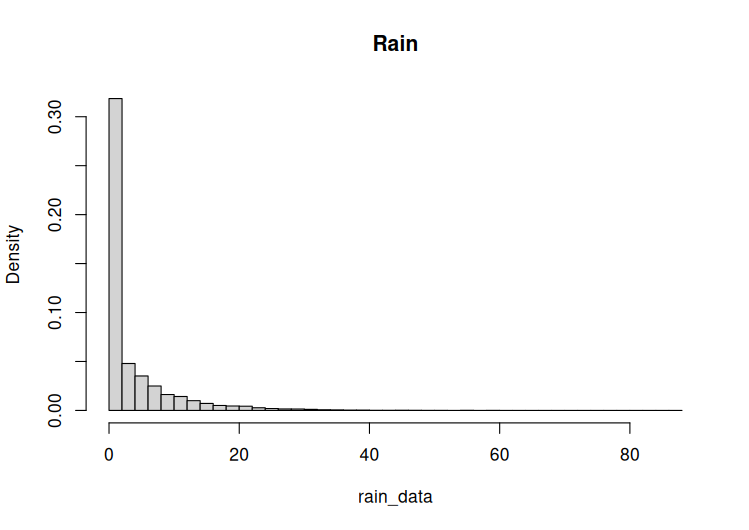
\includegraphics[scale=0.70]{./images/rainhisto.png} 
\end{center}

Dans le cas de rain, on remarque que les données sont concentrées autour de 0 mais qu'elles sont capables de prendre des valeurs très élevées jusqu'à 90.
Il est alors raisonnable de penser qu'après estimation, on va obtenir une valeur de gamma positive ou nulle. En effet, il n'apparait pas de cassure dans la distribution des données.
De plus, les données prennent des valeurs grandes mais perdent rapidement en densité pour celle-ci. Ce qui suggèrerait une valeur de gamma proche de $0$ et positive.

\begin{center}
	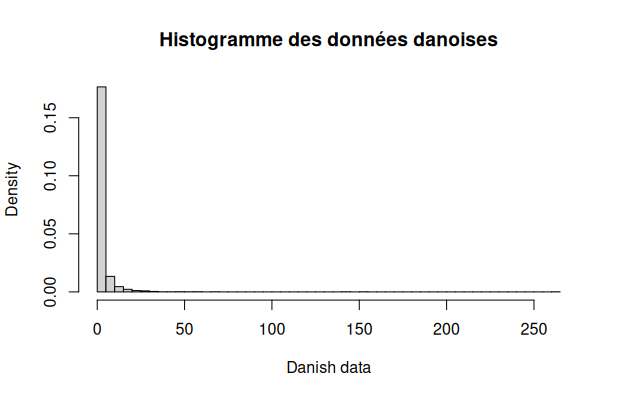
\includegraphics[scale=0.70]{./images/sinistres.png} 
\end{center}

De même, pour les sinistres, on remarque que la majorité des sinistres sont de faible intensité mais qu'il existe des sinistres de grande intensité. On peut donc s'attendre à une valeur de gamma positive ou nulle.

\subsection{Méthode des maxima par bloc}

\subsubsection{Application sur les données de Rain}

Les données étant journalières, on va choisir des blocs de taille 365, comme les données vont de 1914 à 1962, on se retrouve avec 48 blocs de 365 jours.
\\
\\
Via le package \textbf{evd}, on obtient via une estimations par maximum de vraisemblance les paramètres suivants :
\\
$\mu = 40,8$, $\sigma = 9,73$ et $\gamma = 0,107$.
\\
L'estimation des paramètres sont calculées par l'algorithme de Nelder-Mead (voir annexe).
\\
\\
On suppose alors que $\gamma \geq 0$, donc il n’existe pas de valeur maximale finie : la probabilité de très gros maxima décroît mais n'est pas finie, selon un comportement polynomial ou exponentiel ce qui est embettant dans le cas pratique surtout quand on cherche des seuils rarement atteints.
\subsubsection{Application sur les données danish}
On applique la même méthode sur les données de sinistres mais avec une approche légèrement différente puisque les données ne sont pas dans le même format. En effet, on ne dispose pas de données journalières mais l'ensemble des sinistres sur une période de 10 ans. C'est à dire qu'il existe des jours sans sinistres qui ne sont pas comptabilisés.
On regroupe alors les sinistres par mois et on prend le sinistre le plus élevé. On se retrouve alors avec des blocs de taille irrégulière.
\\
\\
Après analyse numérique par maximum de vraisemblance, on obtient les paramètres suivants : $\mu = 8,376$, $\sigma = 5,971$ et $\gamma = 0,623$.
\\
\\
On possède une valeur de gamma positive ce qui renforce l'hypothèse d'une queue lourde pour la distribution du max.

\subsubsection{synthèse sur la méthode des maxima en bloc}

Quand on dispose des données sur une longue période, la méthode des maxima en bloc est efficace. D'autant plus quand on a des données temporelles (journalières, mensuelles, annuelles).
En revanche, elle utilise moins de données ce qui la rend plus difficile à utiliser en pratique. En effet, on ne garde que les maximums et on perd donc une partie des données qui peuvent etre consequents en fonction du choix de $k$.
Par ailleurs, le choix de $k$ est important car il faut choisir un nombre de blocs suffisant pour avoir une estimation fiable mais pas trop grand pour ne pas perdre trop d'informations.

\subsection{Méthode de dépassement de seuil}


\subsubsection{Application sur les données de Rain}

On a calculé la valeur de $\gamma$ par la méthode des maxima en bloc et obtenu une valeur de $\gamma $ positive mais proche de 0. On souhaite s'assurer du signe de $\gamma$
en procédant par la méthode de dépassement de seuil. On va deplus estimer la valeur de $\gamma$ avec l'estimateur de Pickands.
\\
On decide de prendre un seuil correspondant au quantile d’ordre 0,95.
\\
\\
On obtient numériquement : 
$\gamma  = -0.027$
\\
\\
On a obtenu dans la méthode des maxima en bloc une valeur de $\gamma$ postive mais proche de 0,
tandis qu'avec la méthode de dépassement de seuil, on obtient une valeur négative mais tout aussi proche de 0.
\\
Ce qui nous amène à conclure que la valeur de $\gamma$ est de 0.
\\
Autrement dit, la distribution du maximum de pluie suit une loi de Gumbel.
\\
\\
On peut néamoins donner une valeur "seuil" qui nous assurerait que la probabilité de dépasser cette valeur est très faible. 
On calcule alors le quantile de retour pour $T=100$ afin d'avoir une valeur de pluie qui ne devrait pas être dépassée plus d'une fois tous les 100 ans.
\\
\\
Dans notre cas, on obtient alors : $z_t = 98,636$. Autrement dit, une fois tous les 100 ans, on peut s'attendre à avoir une pluie de plus de 98.636 mm.

\subsubsection{Application sur les données danish}

On prend un seuil correspondant au quantile d’ordre 0,95. Apres calcul numérique, on obtient $\sigma = 7.038$ et $\gamma = 0.492$.
\\
On a obtenue une valeur de $\gamma$ positive ce qui renforce l'hypothèse d'une queue lourde pour la distribution du max, ce qui est cohérent avec la méthode des maxima en bloc. On peut pousser l'analyse de gamma en calculant son estimation via l'estimateur de Hill afin d'avoir une valeur plus précise.
\\
\\
On trace alors la courbe de l'estimateur de Hill en fonction de $k$.

\begin{center}
	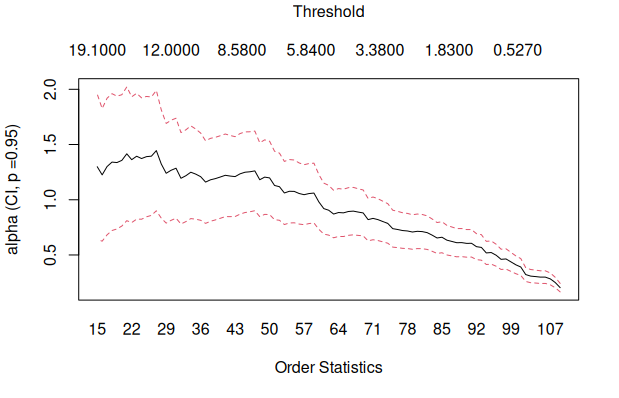
\includegraphics[scale=0.70]{./images/danishsad.png} 
\end{center}

On observe alors un plateau pour k entre 30 et 45. On obtient alors apres estimation numérique une valeur de $\gamma = 0,66$.
\\
On peut alors calculer le quantile de retour pour $T=50$ afin d'avoir une valeur de sinistre qui ne devrait pas être dépassée plus d'une fois tous les 50 ans.
\\
On obtient alors : $z_t = 515,22$. Autrement dit, une fois tous les 50 ans, on peut s'attendre à avoir un sinistre depassant plus de $515,22$.

\subsubsection{Synthèse sur la méthode de dépassement de seuil}
Cette méthode à le bont goût d'exploiter toutes les valeurs supérieures à un seuil, pas seulement un maximum par bloc. Elle utilise donc plus de données.
\\
En revanche le choix du seuil est important car il faut choisir un seuil suffisamment élevé pour ne pas avoir trop peu de données mais pas trop élevé pour ne pas perdre d'informations sur les max. Il faut donc faire le compromis entre le biais et la variance.

\newpage
\section{Annexe}

\subsection{Méthode de Nelder-Mead}

\noindent Le package "evd", que nous avons utilisé pour réaliser les méthodes de dépassement de seuil et des maxima en bloc, utilise l'algorithme de Nelder-Mead pour calculer les paramètres de la fonction limite et ainsi savoir dans quel cas où se trouve : Fréchet, Gumbel ou Weibull. \\

\noindent Nelder-Mead est un algorithme d'optimisation non linéaire, il consiste en la chose suivante dans le cadre des valeurs extrêmes : 
\begin{itemize}
	\item \textbf{Etape 1} : on commence par choisir 3 premiers points $x_1, x_2, x_3$ par une rapide estimation des paramètres $\sigma$, $\mu$ et $\gamma$ de nos données. Ce seront nos points de départs de l'algorithme et ils définissent notre premier simplexe (triangle ici) dans $R^2$.
	\item \textbf{Etape 2} : on calcule ensuite la valeur de la fonction en ces 3 points : f est la fonction GEV généralisée (à définir plus précisément) et on les trie par valeurs décroissantes.
	\item \textbf{Etape 3} : on cherche le centre de gravité $x_0$ de nos premiers points : $x_0 = \frac{x_1 + x_2 + x_3}{3}$.
	\item \textbf{Etape 4} : on fait ensuite une réflexion en calculant $x_r = x_0 + \alpha (x_0 - x_3)$ où $\alpha > 0$ est appelé le coefficient de réflexion
	\item \textbf{Etape 5} : si $f(x_1) \le  f(x_r) \le  f(x_3)$ : on remplace $x_3$ par $x_r$ et on retourne à l'étape 2.
	\item \textbf{Etape 6} : si $f(x_r) \le  f(x_1)$ : on procède à une expansion du simplexe, on calcule $x_3 = x_0 + \gamma(x_r - x_0)$ où $\gamma > 1$. Si $f(x_e) \le  f(x_r) $, on remplace $x_3$ par $x_e$ sinon on remplace $x_3$ par $x_r$ et on retourne à l'étape 2
	\item \textbf{Etape 7} : si $f(x_r) \geq f(x_3)$ : on procède à une contraction du simplexe, on cherche $x_c = x_0 + \rho(x_3 - x_0)$ où $0 < \rho < 0.5 $ . Si $f(x_c) \le  f(x_3)$, on remplace $x_3$ par $x_c$ et on retourne à l'étape 2, sinon on continue jusqu'à l'étape 8.
	\item \textbf{Etape 8} : on effectue une homothétie de rapport $\omega$ et de centre $x_1$ : on remplace ainsi $x_i$ par $x_1 + \omega(x_i - x_1)$ où $0 < \omega < 1$et on retourne à l'étape 2
\end{itemize}

\noindent On répète cela jusqu'à atteinte du critère d'arrêt, en général : $ \sqrt{\sum_{i=1}^{n+1}  \frac{(f_i - \bar{f})^2}{n}} < \epsilon $ où $\bar{f} =\frac{1}{n+1} \sum_{i=1}^{n+1} f_i $ et $ \epsilon $ est un réel proche de 0. \\


\subsection{Codes R}

\noindent Voici un exemple de code R utilisé dans la première section :

\begin{lstlisting}
	# Paramètres
	n <- 1000        # Taille de l'échantillon pour la simulation des lois uniformes
	N <- 10000       # Nombre de simulations pour le maximum
	
	# Simulation des maxima de lois uniformes(0,1)
	set.seed(123)    # fixation de l'aléa
	M_n <- replicate(N, max(runif(n))) # M_n = max / X_n = runif
	
	# Normalisation pour observer la convergence
	Y_n <- n * (1 - M_n)
	
	# Histogramme des valeurs transformées
	hist(Y_n, breaks = 50, probability = TRUE, 
	col = "lightblue", border = "white", ylab = "Densité",
	xlab = expression(Y_n), main = "Max de 1000 lois uniformes")
	
	# Densité théorique de la loi exponentielle (paramètre = 1)
	curve(dexp(x, rate = 1), col = "red", lwd = 2, add = TRUE)
	
	# Légende
	legend("topright", legend = c("Simulation", "Densité théorique : exp(1)"),
	fill = c("lightblue", NA), border = c("white", NA), 
	lty = c(NA, 1), col = c(NA, "red"), lwd = c(NA, 2))
\end{lstlisting}

\begin{lstlisting}
	#################### CODE POUR WOOSTER ####################
	library(ismev)
	library(evd)
	data("wooster")
	
	gev_fit <- fgev(wooster)
	
	mu <- as.numeric(gev_fit$param[1])
	sigma <- as.numeric(gev_fit$param[2])
	gamma <- as.numeric(gev_fit$param[3])
	
	# estimation de gamma avec pickands (juste pour comparer)
	
	x <- sort(wooster)
	n <- length(x)
	k <- floor(0.1 * length(wooster))
	X1 <- x[n - k + 1]
	X2 <- x[n - 2*k + 1]
	X3 <- x[n - 4*k + 1]
	pickands_est <- (1 / log(2)) * log((X1 - X2) / (X2 - X3))
	print(pickands_est)
	
	
	# gamma est < 0 donc on calcule la borne max
	x_max <- mu - sigma / gamma
	
	# Définir la densité de la loi (pour gamma < 0)
	dgev <- function(x, mu, sigma, gamma) {
	  t <- 1 + gamma * ((x - mu) / sigma)
	  dens <- ifelse(t > 0, 
					 (1/sigma) * t^(-1/gamma - 1) * exp(-t^(-1/gamma)), 
					 0)
	  return(dens)
	}
	
	xseq <- seq(min(wooster), max(wooster), length.out = 200)
	
	# PLOT   
	
	hist(wooster,main = "Histogram de wooster" ,breaks = 60, probability = TRUE, col = "lightgray")
	
	lines(xseq, dgev(xseq, mu, sigma, gamma), col = "blue", lwd = 2)
	
	
	abline(v = x_max, col = "red", lwd = 2, lty = 2)
	legend("topright", legend = paste("x_max =", round(x_max, 2)), col = "red", lwd = 2, lty = 2)
	
	# plot plus détaillé
	plot(gev_fit)



	
\end{lstlisting}

\begin{lstlisting}
	#################### CODE POUR RAIN ####################
	library(ismev)
	library(evd)
	data(rain)
	rain_data <- rain

	# seuil	
	threshold <- quantile(rain_data, probs = 0.95)
	gpd_result <- gpd.fit(rain_data, threshold)

	# on stocke la parametre d'échelle et de forme
	sigma <- gpd_result$mle[1]
	gamma <- gpd_result$mle[2]
	SE <- gpd_result$se[2]
	IC <- c(gamma - 1.96 * SE, gamma + 1.96 * SE)    # contient 0 (oups)


	# On code la fonction de pareto généralisée parametre echel sigma et de forme gamma
	pareto <- function(x, gamma, sigma) {
	  if (gamma == 0) {
		return(1/sigma * exp(-x/sigma))
	  } else {
		return(1/sigma * (1 + gamma * x/sigma)^(-1/gamma - 1))
	  }
	}

	# on trace l'histogramme des données
	hist(rain_data, breaks = 50, freq = FALSE, main = "Rain")

	# on trace l'histogramme des données en excés par rapport au seuil et la loi de pareto
	hist(rain_data[rain_data > threshold] - threshold, breaks = 50, freq = FALSE, main = "Rain Excesses et densité de Pareto")

	# on trace la loi de gpd avec les paramètres estimés
	xseq <- seq(min(rain), max(rain), length.out = 200)
	lines(xseq, pareto(xseq, gamma, sigma),col='red', lwd=2)



	# pour le qq-plot et residus
	gpd.diag(gpd_result)

\end{lstlisting}
\end{document}